\documentclass[twoside,openright,titlepage,fleqn,
	headinclude,11pt,a4paper,BCOR5mm,footinclude
	]{scrbook}
%--------------------------------------------------------------
        \newcommand{\myTitle}{Progettazione e Analisi di Algoritmi\xspace}
% use the right myDegree option
\newcommand{\myDegree}{Corso di Laurea Magistrale in Informatica\xspace}
%\newcommand{\myDegree}{
	%Corso di Laurea Specialistica in Scienze e Tecnologie 
	%dell'Informazione\xspace}
\newcommand{\myName}{Massimo Nocentini\xspace}
\newcommand{\myProf}{Donatella Merlini\xspace}
\newcommand{\myOtherProf}{Maria Cecilia Verri\xspace}
\newcommand{\mySupervisor}{Nome Cognome\xspace}
\newcommand{\myFaculty}{
	Facolt\`a di Scienze Matematiche, Fisiche e Naturali\xspace}
\newcommand{\myDepartment}{
	Dipartimento di Sistemi e Informatica\xspace}
\newcommand{\myUni}{\protect{
	Universit\`a degli Studi di Firenze}\xspace}
\newcommand{\myLocation}{Firenze\xspace}
\newcommand{\myTime}{Anno Accademico 2012-2013\xspace}
\newcommand{\myVersion}{Version 0.1\xspace}

%--------------------------------------------------------------
\usepackage[latin1]{inputenc} 
\usepackage[T1]{fontenc} 
\usepackage[square,numbers]{natbib} 
\usepackage[fleqn]{amsmath}  
\usepackage[english]{babel}
\usepackage{ae,aecompl}
\usepackage[pdftex]{graphicx}
\usepackage{latexsym}
\usepackage{amsmath, amsthm, amssymb}
\usepackage{rotating}
\usepackage{boxedminipage}
\usepackage{multicol}
\usepackage{rotating}

%--------------------------------------------------------------
\usepackage{dia-classicthesis-ldpkg} 
%--------------------------------------------------------------
% Options for classicthesis.sty:
% tocaligned eulerchapternumbers drafting linedheaders 
% listsseparated subfig nochapters beramono eulermath parts 
% minionpro pdfspacing
\usepackage[eulerchapternumbers,subfig,beramono,eulermath,
	parts]{classicthesis}
%--------------------------------------------------------------
\newlength{\abcd} % for ab..z string length calculation
% how all the floats will be aligned
\newcommand{\myfloatalign}{\centering} 
\setlength{\extrarowheight}{3pt} % increase table row height
\captionsetup{format=hang,font=small}
%--------------------------------------------------------------
% Layout setting
%--------------------------------------------------------------
\usepackage{geometry}
\geometry{
	a4paper,
	ignoremp,
	bindingoffset = 1cm, 
	textwidth     = 13.5cm,
	textheight    = 21.5cm,
	lmargin       = 3.5cm, % left margin
	tmargin       = 4cm    % top margin 
}
%--------------------------------------------------------------
\usepackage{listings}
\usepackage{hyperref}
\usepackage{pdfpages}
% My Theorem
\newtheorem{oss}{Observation}[section]
\newtheorem{exercise}{Exercise}[section]
\newtheorem{thm}{Theorem}[section]
\newtheorem{cor}[thm]{Corollary}

\newtheorem{lem}[thm]{Lemma}

\newcommand{\vect}[1]{\boldsymbol{#1}}

% questo comando e' relativo alle correzioni che puo
% apportare il prof se lo desidera.
\newcommand{\prof}[1]{\boldsymbol{#1}}

% instead of boldsymbol I can use the arrow above the letter with
%\newcommand{\vect}[1]{\vec{#1}}

% page settings
% \pagestyle{headings}
%--------------------------------------------------------------
\begin{document}
\frenchspacing
\raggedbottom
\pagenumbering{roman}
\pagestyle{plain}
%--------------------------------------------------------------
% Frontmatter
%--------------------------------------------------------------
%--------------------------------------------------------------
% titlepage.tex (use thesis.tex as main file)
%--------------------------------------------------------------
\begin{titlepage}
	\begin{center}
   	\large
      \hfill
      \vfill
      \begingroup
			\spacedallcaps{\myUni} \\ 
			\myFaculty \\
			\myDegree \\ 
			\vspace{0.5cm}
         
\includegraphics[scale=.065]{logo/unifi}\\
         \vspace{0.5cm}    
         %% -------put here the type of document---ie: Tesi di Laurea
         Elaborato d'Esame
      \endgroup 
      \vfill 
      \begingroup
      	\color{Maroon}\spacedallcaps{\myTitle} \\ \bigskip
      \endgroup
      \spacedlowsmallcaps{\myName}
      \vfill  
      % Professoresse:
      \itshape{\myProf}\\\itshape{\myOtherProf}
      \vfill  
      \myTime
      \vfill                      
	\end{center}        
\end{titlepage}   
%--------------------------------------------------------------
% back titlepage
%--------------------------------------------------------------
   \newpage
	\thispagestyle{empty}
	\hfill
	\vfill
	\noindent\myName: 
	\textit{\myTitle,} 
	\myDegree, \textcopyright\ \myTime
%--------------------------------------------------------------
% back titlepage end
%--------------------------------------------------------------
\pagestyle{scrheadings}
%--------------------------------------------------------------
% Mainmatter
%--------------------------------------------------------------
\pagenumbering{arabic}

% settings for the lstlisting environment
\lstset{
	language = R
	, numbers = left 
	, basicstyle=\sffamily%\footnotesize
%	, frame=single
	, tabsize=2
	, captionpos=b
	, breaklines=true
	, showspaces=false
	, showstringspaces=false
}

\tableofcontents

\newpage

\newpage

\subsection*{Text contents}
All the text content is distributed under:\\
\textbf{ This work is licensed under the Creative Commons Attribution,
  NonCommercial, ShareAlike 3.0 Unported License. To view a
  copy of this license, visit\\
  \href{http://creativecommons.org/licenses/by-nc-sa/3.0/}{http://creativecommons.org/licenses/by-nc-sa/3.0/}\\
  or send a letter to Creative Commons, 444 Castro Street, Suite 900,
  Mountain View, California, 94041, USA.}

\begin{center}
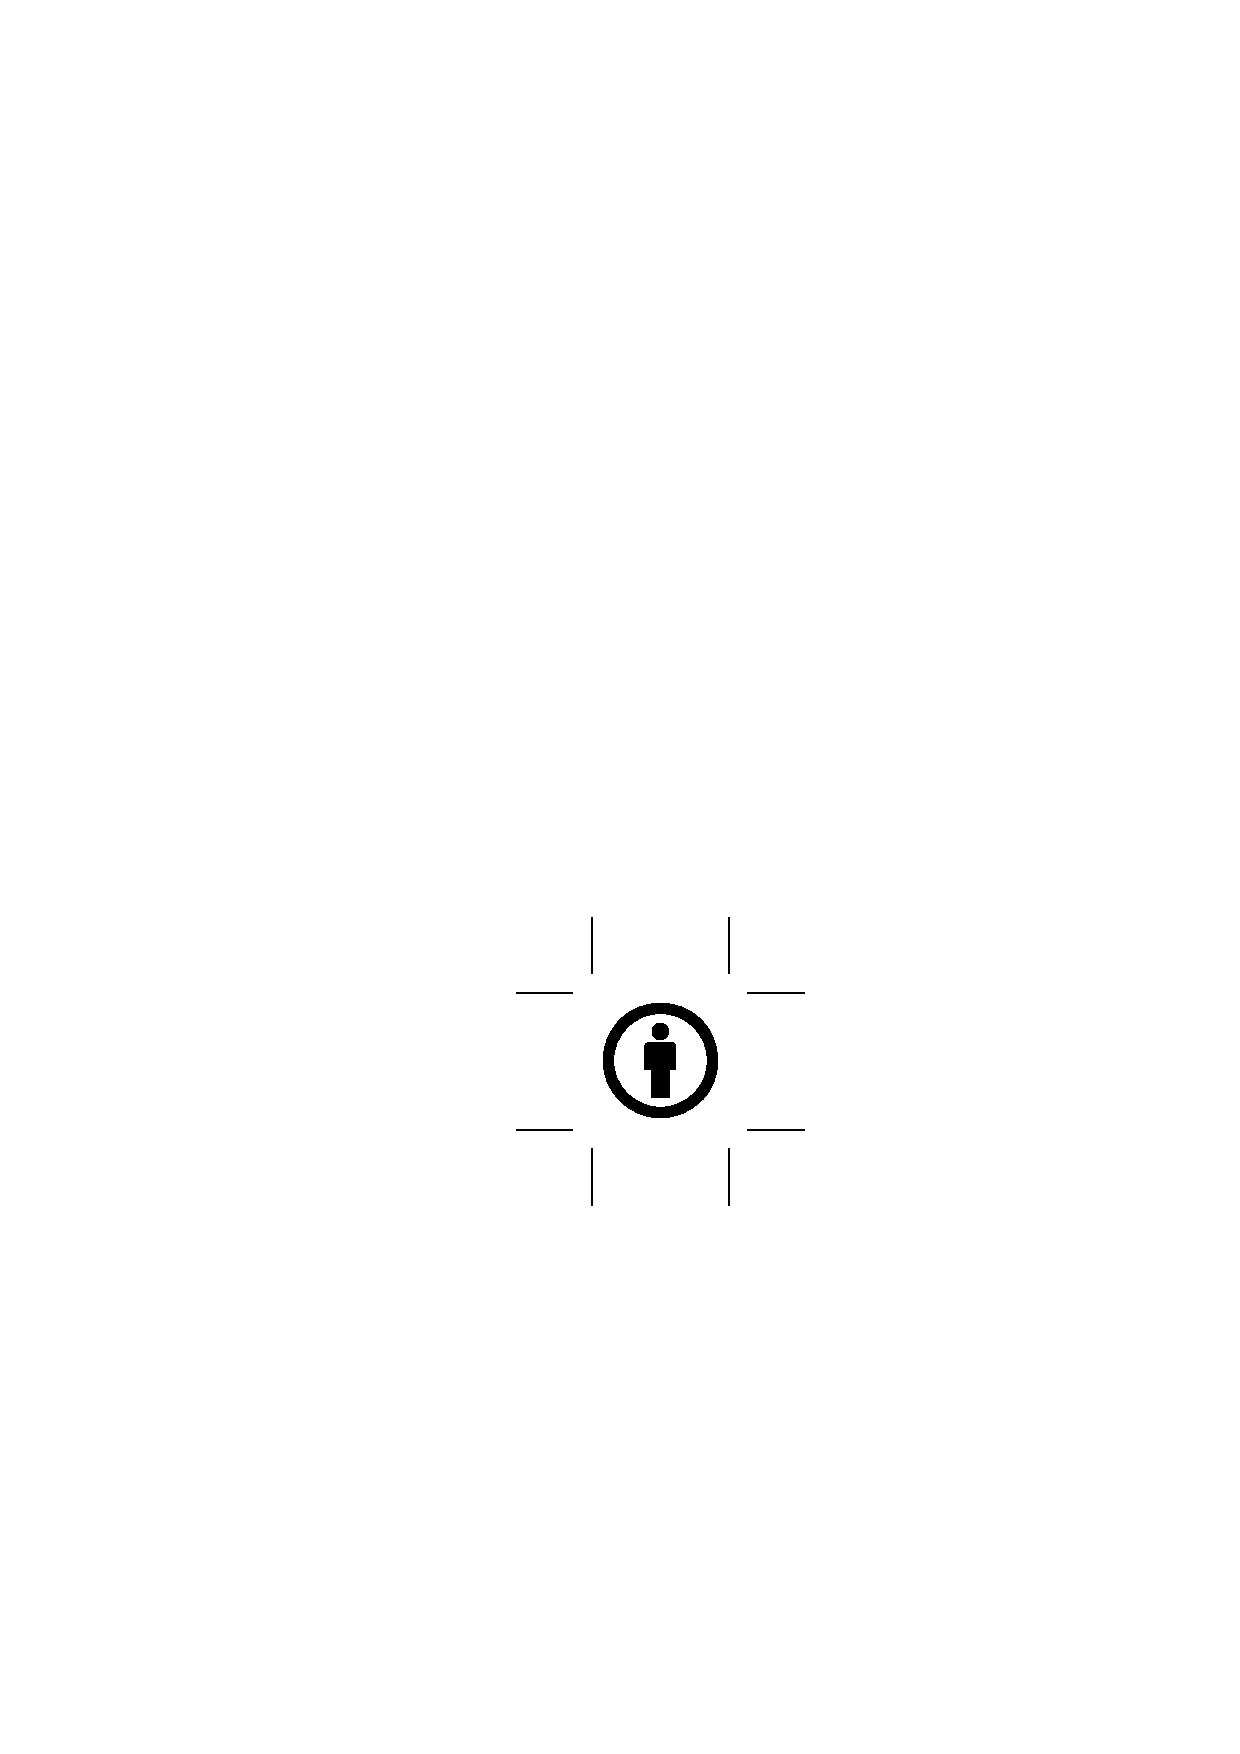
\includegraphics{cc-icons-eps/by}

\includegraphics{cc-icons-eps/cc}
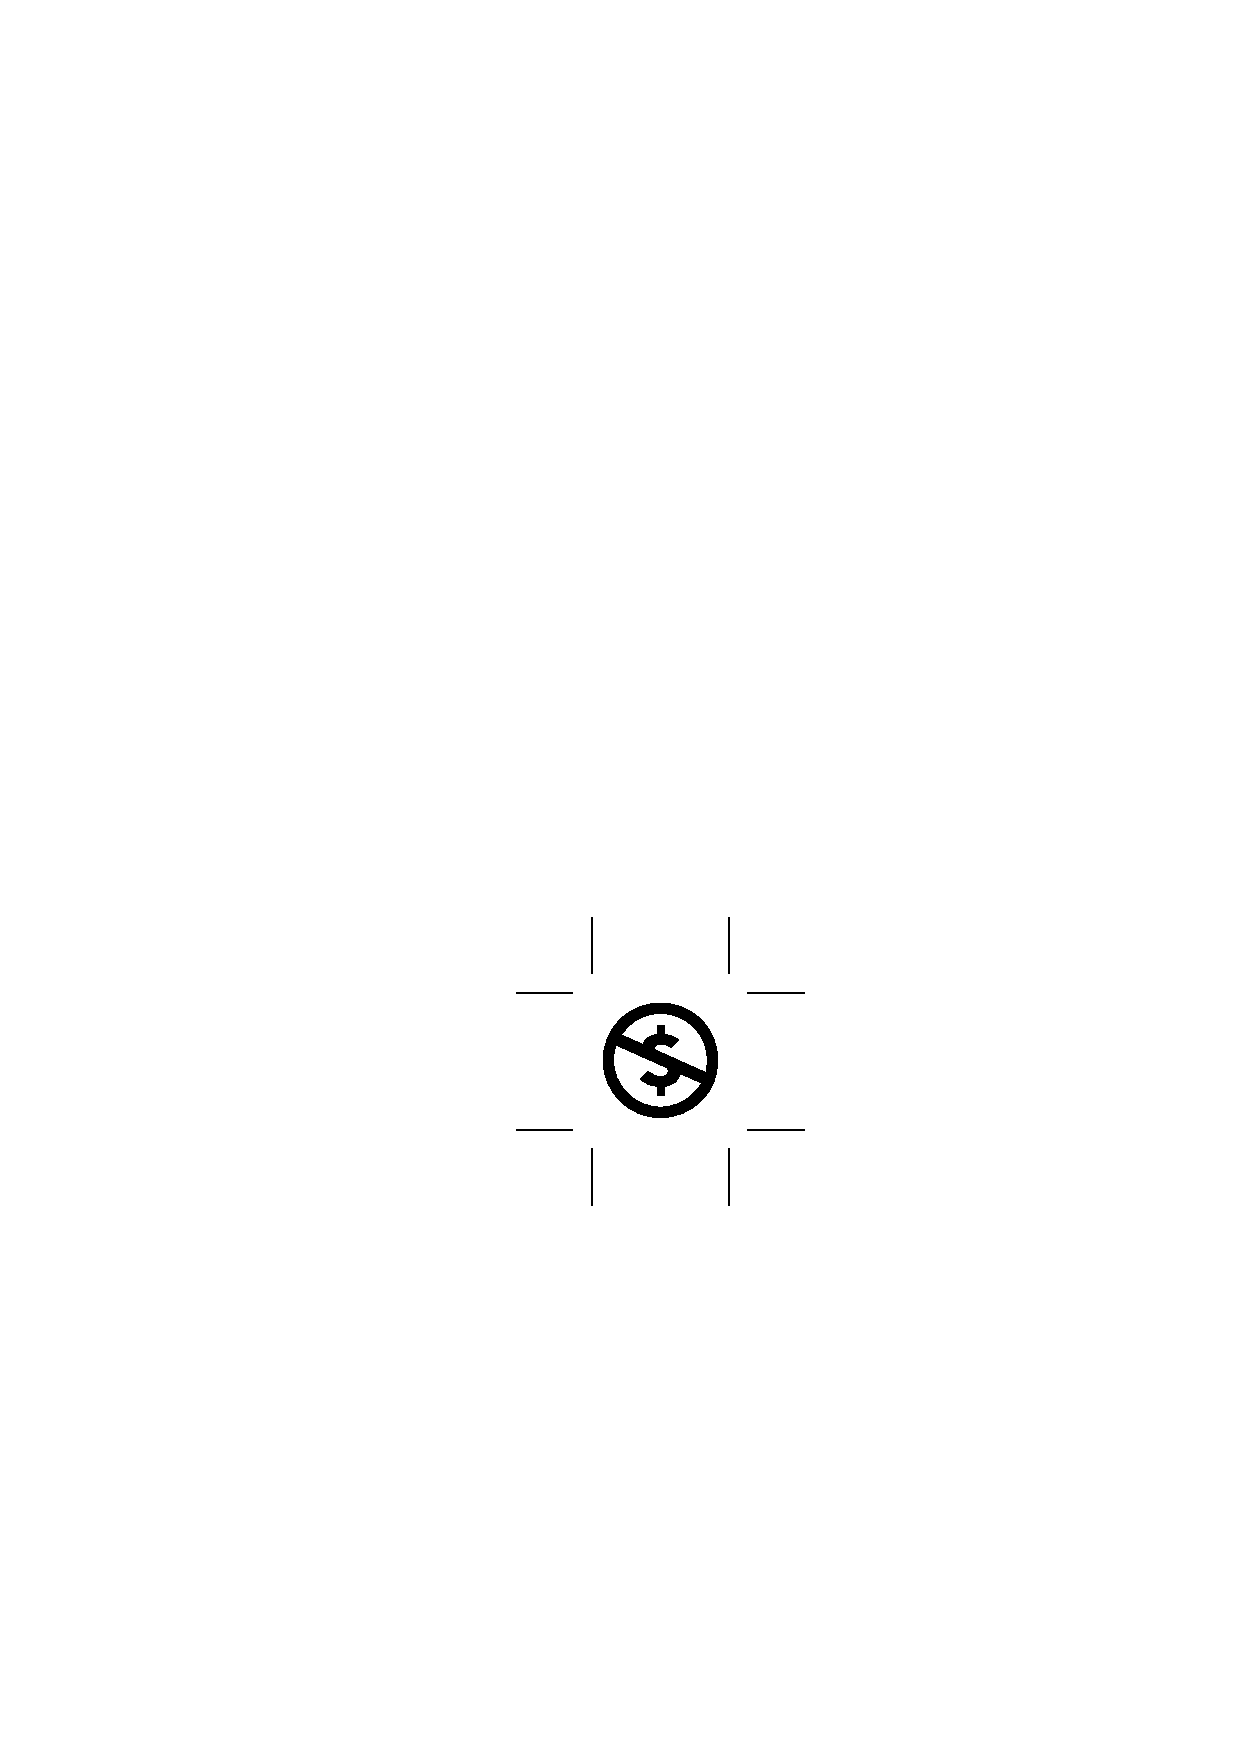
\includegraphics{cc-icons-eps/nc}
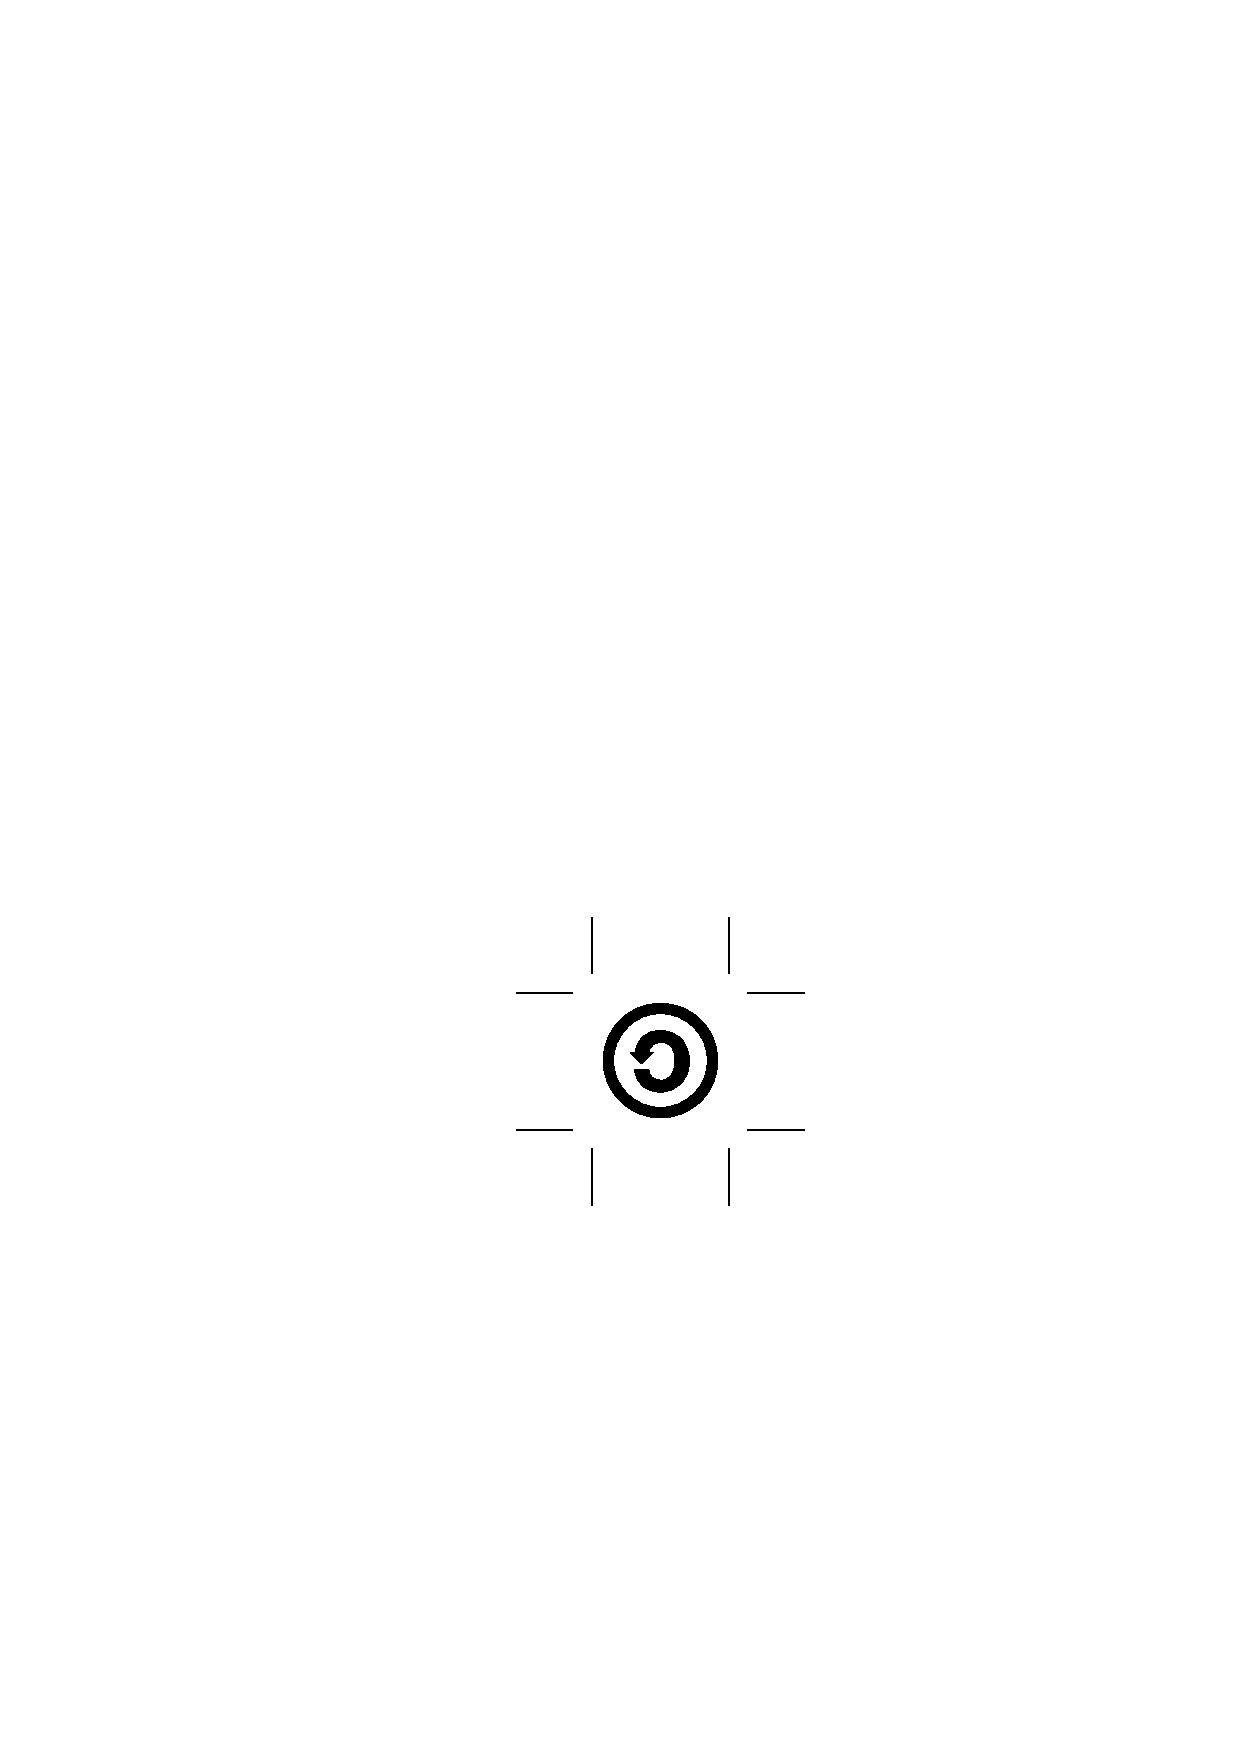
\includegraphics{cc-icons-eps/sa}
\end{center}

\subsection*{Sources}
All sources are distributed under, where the word ``Software'' is
referred to all of the sources that are present in this work: \\
\textbf{
  Copyright (c) 2011 Massimo Nocentini\\
  Permission is hereby granted, free of charge, to any person
  obtaining a copy of this software and associated documentation files
  (the "Software"), to deal in the Software without restriction,
  including without limitation the rights to use, copy, modify, merge,
  publish, distribute, sublicense, and/or sell copies of the Software,
  and to permit persons to whom the Software is furnished
  to do so, subject to the following conditions:\\
  The above copyright notice and this permission notice shall be
  included in all
  copies or substantial portions of the Software.\\
  THE SOFTWARE IS PROVIDED "AS IS", WITHOUT WARRANTY OF ANY KIND,
  EXPRESS OR IMPLIED, INCLUDING BUT NOT LIMITED TO THE WARRANTIES OF
  MERCHANTABILITY, FITNESS FOR A PARTICULAR PURPOSE AND
  NONINFRINGEMENT. IN NO EVENT SHALL THE AUTHORS OR COPYRIGHT HOLDERS
  BE LIABLE FOR ANY CLAIM, DAMAGES OR OTHER LIABILITY, WHETHER IN AN
  ACTION OF CONTRACT, TORT OR OTHERWISE, ARISING FROM, OUT OF OR IN
  CONNECTION WITH THE SOFTWARE OR THE USE OR OTHER DEALINGS IN THE
  SOFTWARE.  }


\part{Analysis part}

\chapter{Lectures notes}
Rewrite here the content of the lectures during the classes.

\chapter{Sequential search simulation}

We've repeated the simulation for the \emph{sequential search} problem
as did during the class. We want to study the mean of checks performed
by the sequential search algorithm before the desired element is
found in the given permutation. After we compare the mean of checks
obtained by simulation with the theoretical mean value for the same
input dimension.

The sequential search algorithm cited above is a very simple searching
method: it consume a permutation of integer of a fixed dimension $n$
and a target integer; produce true if the target belongs to the given
permutation, else otherwise (in our case we augment the information
returned with the number of checks needed in the run). The searching
strategy consists of starting from the very left and moving one step
to right every time the target is missed.

\section{Implementation}

We don't report here the description for the implementation of the
sequential search algorithm because is very simple. Instead, we focus
the explanation on the main simulation procedure.

The simulation function consume three parameters:
\begin{itemize}
\item $numdimensions$, the number of dimensions that we would like to
  test;
\item $interval$, the multiplier to build the permutation vector to be
  used during the search;
\item $attempts$, the number of application of the sequential search
  algorithm to a given permutation.
\end{itemize}
We use the number of dimensions $numdimensions$ to build a vector
$dimensions$ such that both of the following hold:
\begin{displaymath}
  \begin{split}
    length(dimensions)&=numdimensions \\
    dimensions[i]&=i * interval \quad \forall i \in \{1,\ldots,numdimensions\}
  \end{split}
\end{displaymath}
For a given dimension $n \in \{interval, 2*interval,
\ldots,numdimensions*interval\}$, we sample a permutation of integers
from $\{1,\ldots,n\}$ using the uniform distribution. For each
permutation we apply the sequential search algorithm: the number of
application is proportional to $n$ (specifically $2n$) and after every
application we record the number of checks needed to hit the target.
When we run out all the iterations we compute the mean and the
variance of the checks, storing them into auxiliary vectors.

\section{Results}

In \autoref{tab:sequential-search-table-result} we report a summary
table for a simulation invoked with arguments $numdimensions=50,
interval=20, attempts=50$.
\begin{table}[ht]
  \caption{Sequential search summary}
  \label{tab:sequential-search-table-result}
  \begin{center}
    \rotatebox{90}{
      \begin{tabular}{rrrrrrrrrr}
        \hline
        & dimensions & theo means & means & theo vars & vars
        & theo var of vars & var of vars & stand. means & stand. vars \\ 
        \hline
        1 & 20.00 & 10.50 & 10.66 & 33.25 & 34.34 & 877.80 & 975.55 & 1.22 & 1.64 \\ 
        2 & 40.00 & 20.50 & 20.65 & 133.25 & 135.02 & 14177.80 & 14994.21 & 0.82 & 0.94 \\ 
        3 & 60.00 & 30.50 & 30.48 & 299.92 & 302.46 & 71900.02 & 74572.74 & -0.10 & 0.74 \\ 
        4 & 80.00 & 40.50 & 41.09 & 533.25 & 531.28 & 227377.80 & 221994.03 & 2.28 & -0.37 \\ 
        5 & 100.00 & 50.50 & 50.52 & 833.25 & 833.01 & 555277.80 & 553196.84 & 0.07 & -0.03 \\ 
        6 & 120.00 & 60.50 & 60.13 & 1199.92 & 1189.70 & 1151600.02 & 1122368.13 & -1.18 & -1.04 \\ 
        7 & 140.00 & 70.50 & 70.42 & 1633.25 & 1621.51 & 2133677.80 & 2078575.00 & -0.22 & -0.95 \\ 
        8 & 160.00 & 80.50 & 79.80 & 2133.25 & 2155.97 & 3640177.80 & 3782358.53 & -1.92 & 1.51 \\ 
        9 & 180.00 & 90.50 & 91.06 & 2699.92 & 2696.73 & 5831100.02 & 5837985.82 & 1.44 & -0.18 \\ 
        10 & 200.00 & 100.50 & 100.26 & 3333.25 & 3315.86 & 8887777.80 & 8760281.48 & -0.59 & -0.82 \\
        ... &  &  & &  & & & &  &  \\ 
        41 & 820.00 & 410.50 & 409.84 & 56033.25 & 56005.31 & 2511768877.80 & 2520823155.84 & -0.80 & -0.16 \\ 
        42 & 840.00 & 420.50 & 419.93 & 58799.92 & 59131.53 & 2765932400.02 & 2833053962.68 & -0.68 & 1.83 \\ 
        43 & 860.00 & 430.50 & 429.49 & 61633.25 & 61801.47 & 3038913677.80 & 3061925029.95 & -1.20 & 0.89 \\ 
        44 & 880.00 & 440.50 & 441.59 & 64533.25 & 64686.44 & 3331619377.80 & 3349812105.46 & 1.27 & 0.79 \\ 
        45 & 900.00 & 450.50 & 448.81 & 67499.92 & 67476.72 & 3644977500.02 & 3620068539.03 & -1.95 & -0.12 \\ 
        46 & 920.00 & 460.50 & 461.97 & 70533.25 & 70360.59 & 3979937377.80 & 3963315767.79 & 1.68 & -0.83 \\ 
        47 & 940.00 & 470.50 & 470.75 & 73633.25 & 73791.33 & 4337469677.80 & 4381479940.27 & 0.28 & 0.74 \\ 
        48 & 960.00 & 480.50 & 481.49 & 76799.92 & 76684.82 & 4718566400.02 & 4704539498.17 & 1.11 & -0.52 \\ 
        49 & 980.00 & 490.50 & 490.41 & 80033.25 & 80176.91 & 5124240877.80 & 5142289190.74 & -0.10 & 0.63 \\ 
        50 & 1000.00 & 500.50 & 500.43 & 83333.25 & 83210.10 & 5555527777.80 & 5524755813.88 & -0.08 & -0.52 \\ 
        \hline
      \end{tabular}
    }
  \end{center}
\end{table}

We've used the standardized means to plot them againts the normal
distribution in order to verify the Central Limit Theorem in
\autoref{fig:sequential-search-standardized-means}. The dotted curve
represent the normal distribution, the blue one represent the sampling
means distribution instead.
\begin{figure}[htb]
\centering
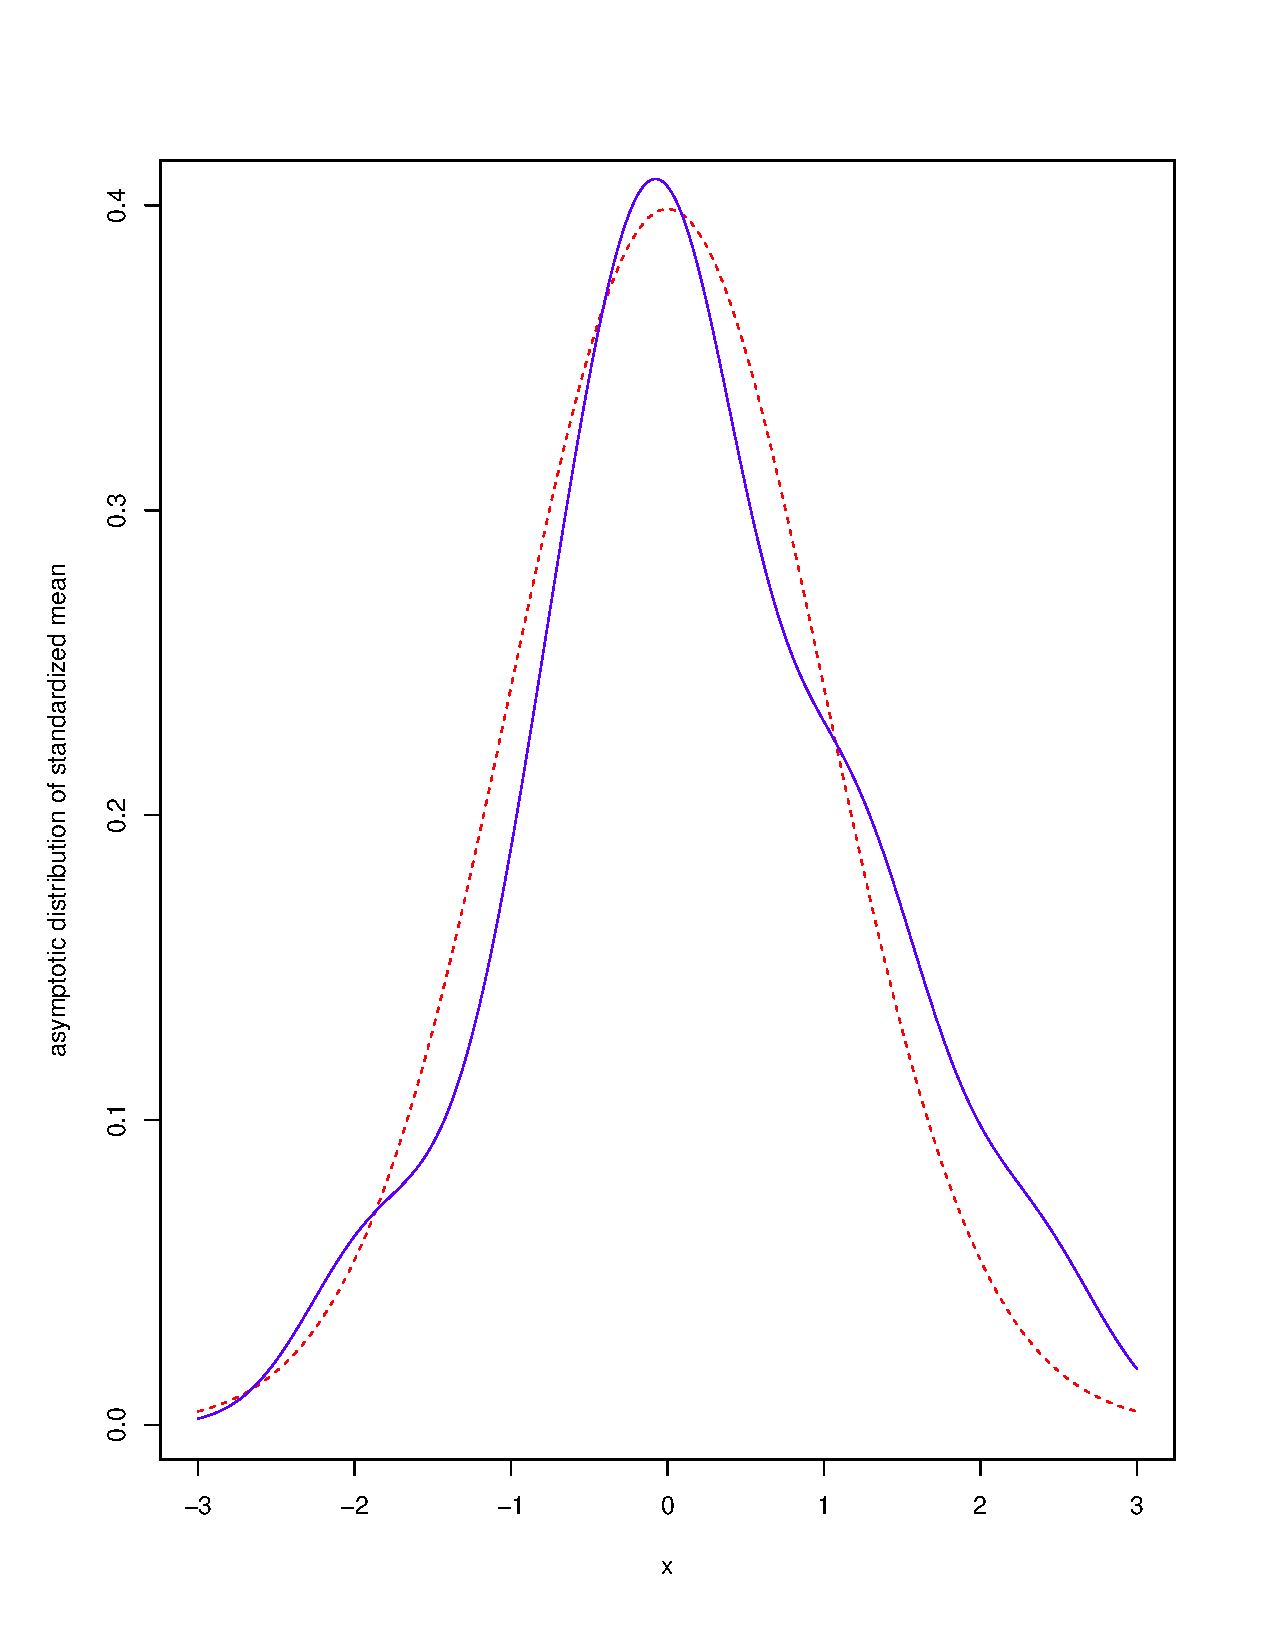
\includegraphics[height=13cm,width=13cm]{pictures/sequential-search-asymtotic-behaviour-of-standardized-means.pdf}
\caption{Plot of standardized means}
\label{fig:sequential-search-standardized-means}
\end{figure}

Also we've build a second plot with a regression of the sampling means in
\autoref{fig:sequential-search-means-regression}. The red line is
drawn after computing the intercept and the coefficient using an
hybrid model. Our attempt to explain the data consists of a mixture up
to the second degree, as follow:
\begin{displaymath}
  \begin{split}
    dims &= \sum_{i}^{n}{dimensions[i]}\\
    means &= \sum_{i}^{n}{mean[i]}\\
    dim\_squares &= \sum_{i}^{n}{dimensions[i]^2}\\
    mean\_squares &= \sum_{i}^{n}{means[i]^2}\\
    dim\_mean &= \sum_{i}^{n}{means[i] * dimensions[i]}\\
    intercept &= \frac{dim\_squares * means - dims *
      dim\_mean}{n*dim\_squares - dims^2}\\
    coefficient &= \frac{n * dim\_mean - dims * means} {n*dim\_squares-dims^2}
  \end{split}
\end{displaymath}
hence the red line is defined $means = coefficient*dimensions + intercept$.
\begin{figure}[htb]
\centering
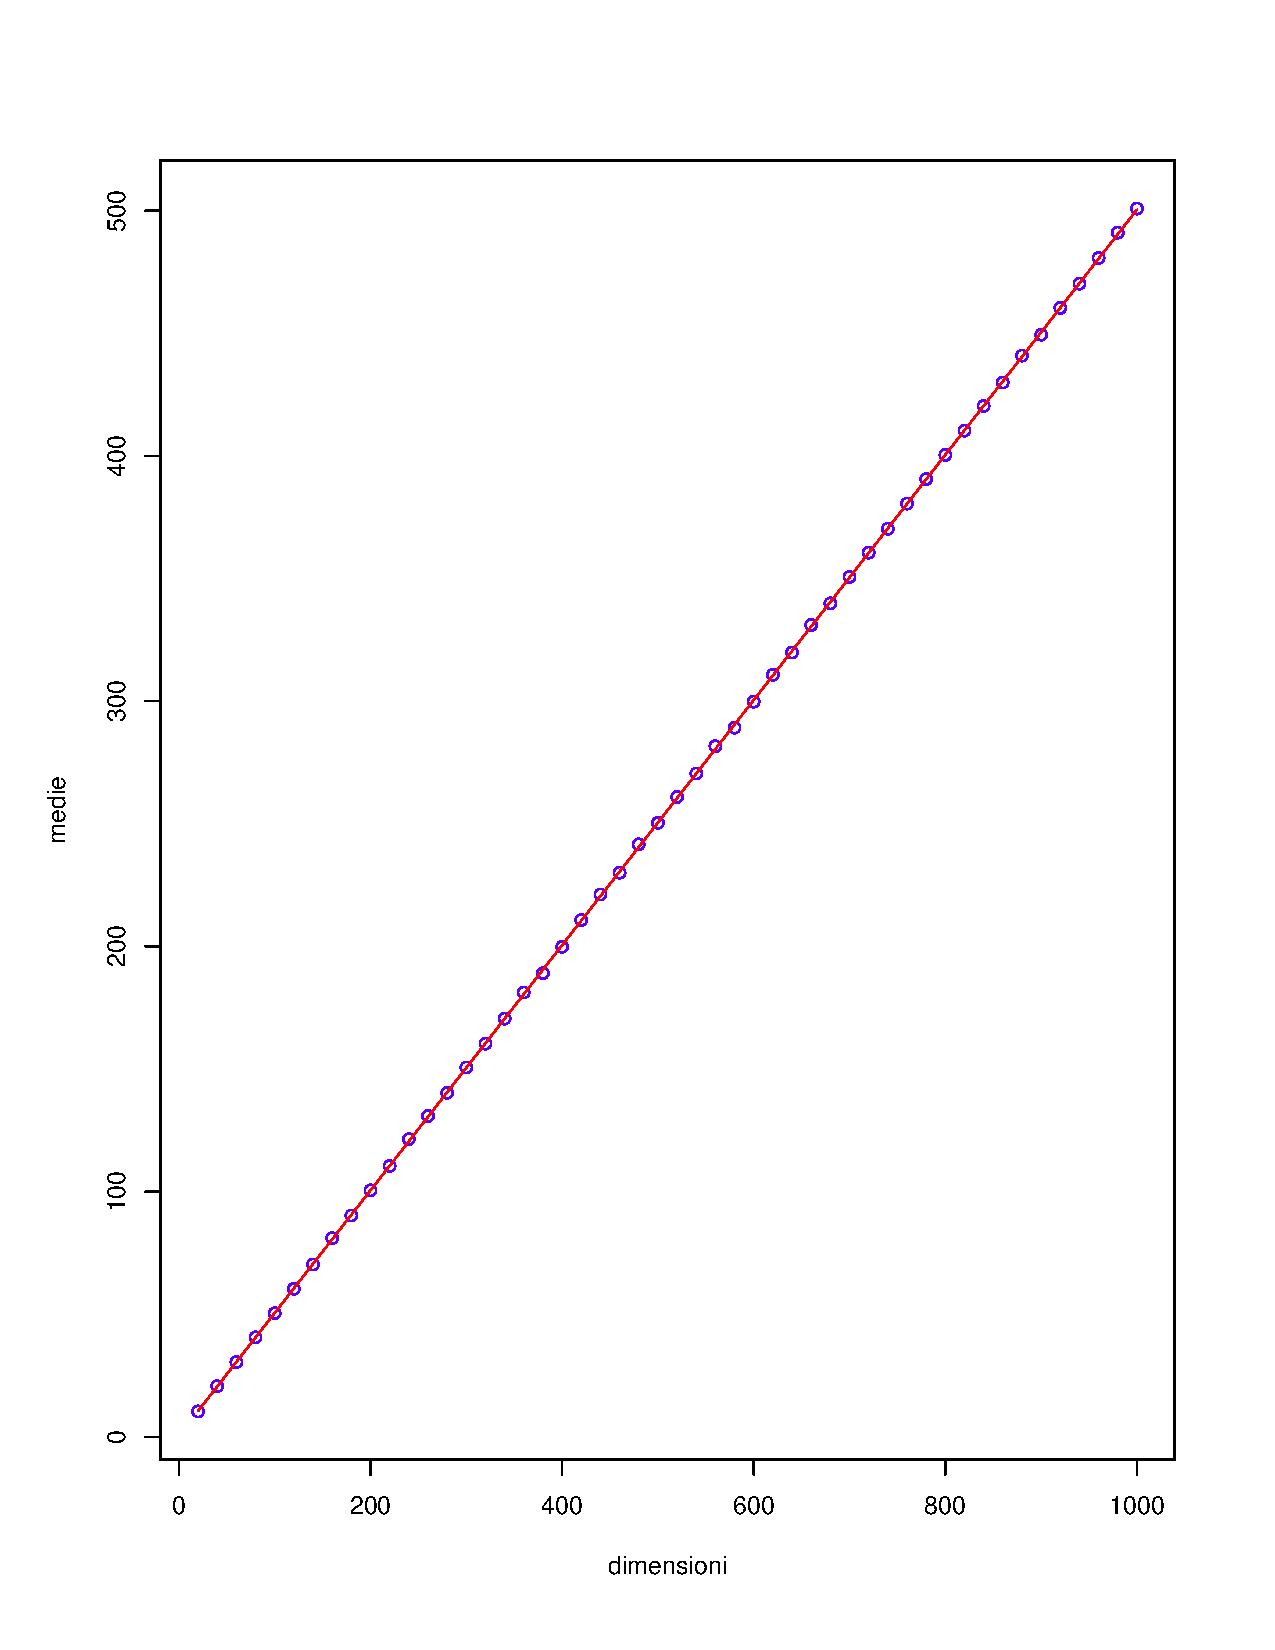
\includegraphics[height=13cm,width=13cm]{pictures/sequential-search-mean-regression-of-sequential-search.pdf}
\caption{Plot of means regression}
\label{fig:sequential-search-means-regression}
\end{figure}





\chapter{Generating binary trees at random}
Explain the project and what we want to accomplish.

\section{Atkinson and Sack algorithm}
Describe briefly the algorithm here.

\section{Implementation using R}

\begin{lstlisting}

  generate.tree <- function(number_of_nodes){

    word_dimension <- 2 * number_of_nodes
    
    universe <- 1:word_dimension
    sample <- sample(universe, size=number_of_nodes)
    w = rep(0, word_dimension)
    for (i in 1:word_dimension) {
      w[i] <- ifelse(any(sample == i), 1, -1)
    }
    
    phi=phi(w)
    list(word=w, phi=phi, as_brackets = brackets_of_word(phi))
  }

  split.word <- function(w){
    if(length(w) == 0)
    return(list(u=c(), v=c()))
    
    u_index_set <- 1:match(0, cumsum(w))
    list(u=w[u_index_set], v=w[-u_index_set])
  }

  phi <- function(w){
    if(length(w) == 0)
    return(w)
    
    split <- split.word(w) 
    
    if(all(cumsum(split$u) > -1)){
      return (c(split$u, phi(split$v)))
    }
    else{
      t = split$u[-c(1, length(split$u))]
      return (c(1, phi(split$v), -1, -t))
    }
  }
\end{lstlisting}

\part{Algorithms part}

\chapter{Divide et impera}
Put here some exercises on some topics of interest.

\chapter{Appendix}

\section{Original article about random binary trees generation}

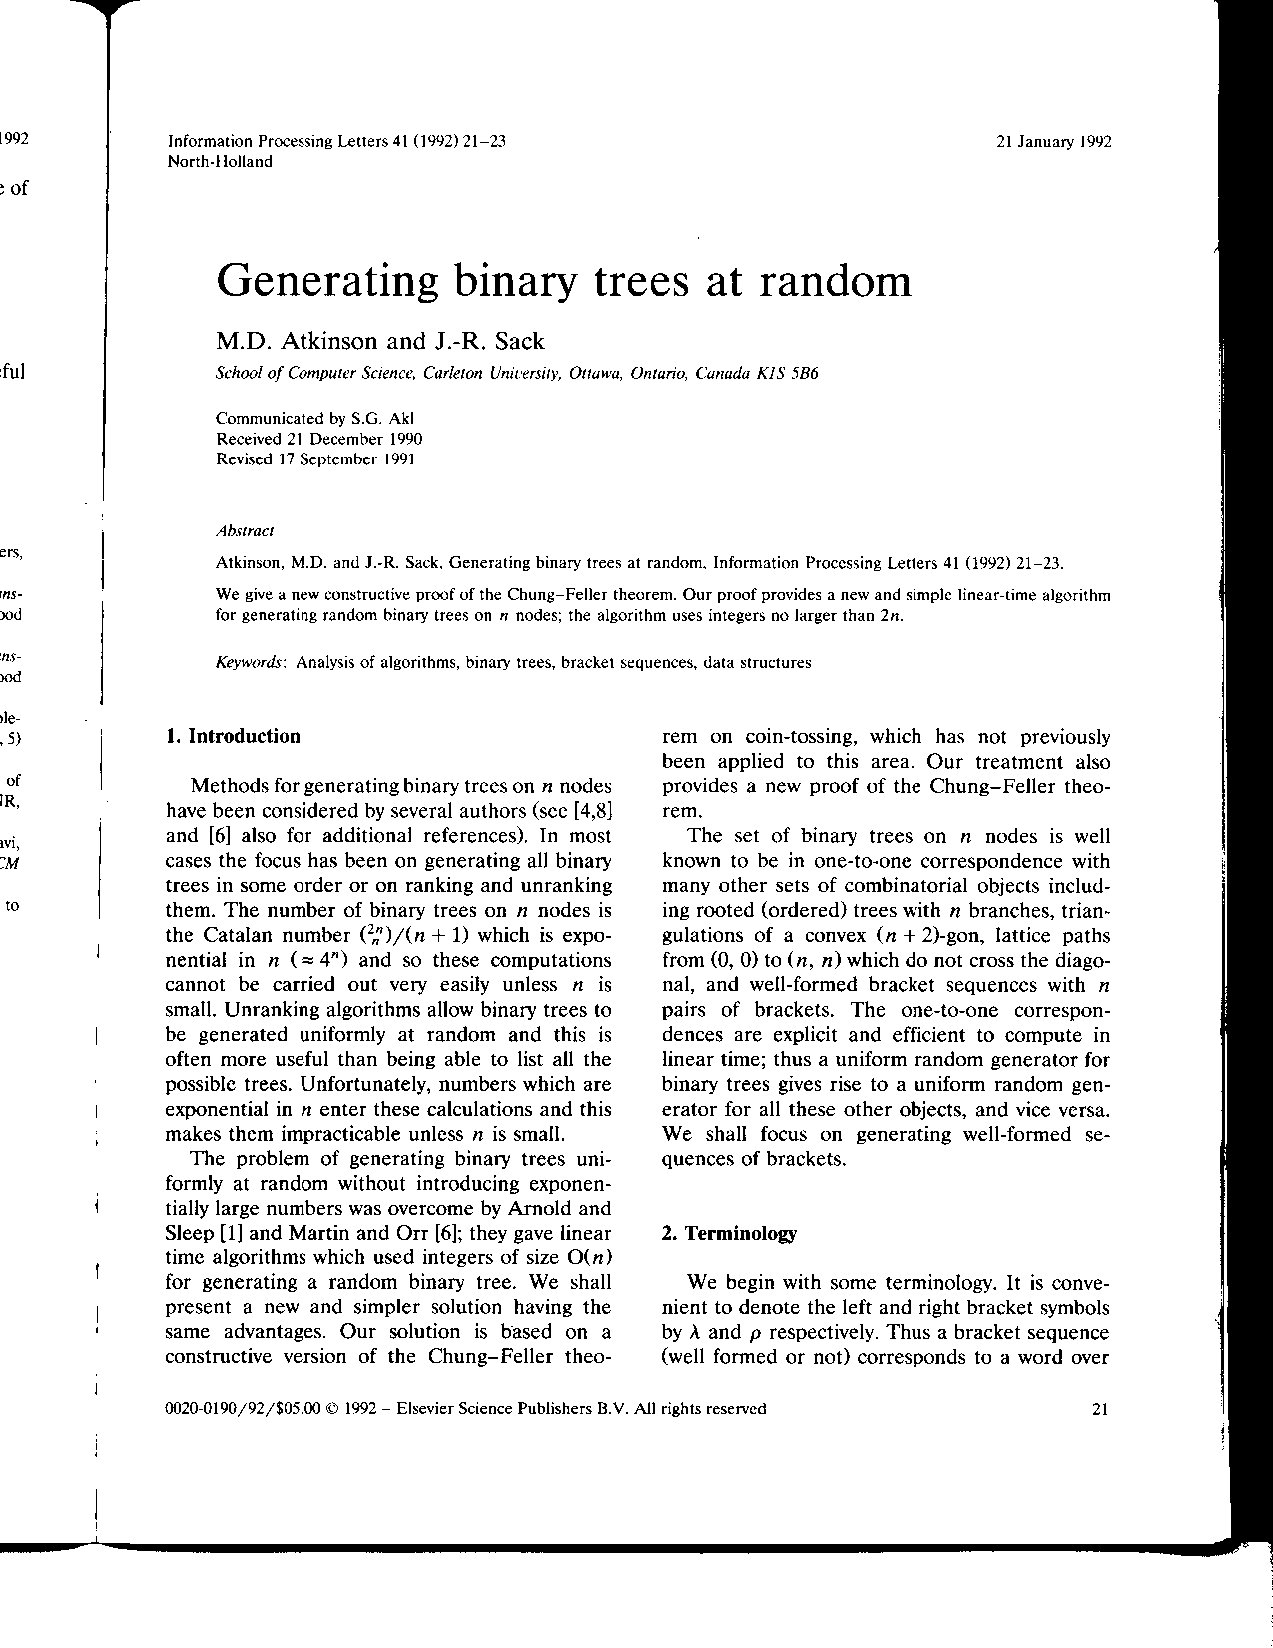
\includepdf[pages={-}]{atkinson-sack-original-article.pdf}

% \section{Full code for random binary trees generation}
% The following block contains the functions written in \emph{R} to
% implement the algorithms related to the generation of binary
% trees. Those functions allow to generate the outputs attached in the
% previous chapters:
% \lstinputlisting{random-trees-generation/generator.R}

% \section{Full code for trees analysis and dot representation}
% The following block contains the functions written in \emph{OCaml} to
% implement the algorithms related to the analysis of the generated
% trees and its dot representation:
% \lstset{language=ML}
% \lstinputlisting{trees-generation-ocaml/main.ml}






\end{document} 
